\chapter{Methodology}
	\section{Agile Method as Software Development Model}
	The development of StudyBug followed the Agile software development methodology. Agile was chosen because the project emphasized user experience, iterative design, and continuous improvement. Since the application includes multiple interactive features such as scheduling, focus timers, task management, quiz generation, and aesthetic customization, Agile allowed these components to be developed and refined incrementally.

	The Agile approach enabled frequent evaluation of progress, early detection of issues, and flexibility in incorporating feedback. Each iteration (sprint) focused on delivering a functional and usable version of the application, which was then enhanced in subsequent iterations.

	\begin{figure}[h]
		\centering
			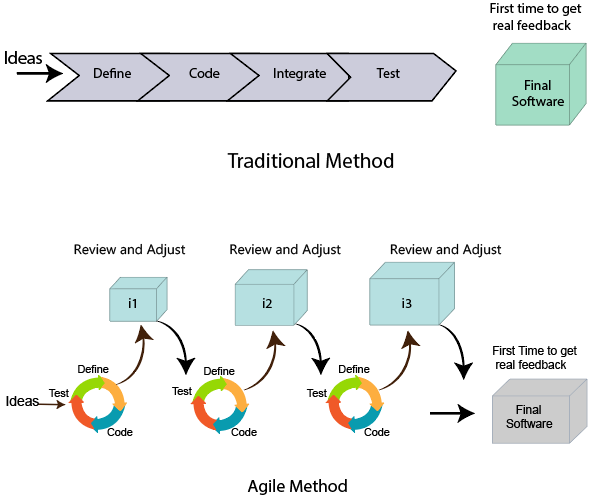
\includegraphics[width=0.8\textwidth]{img/agilem.png}
			\caption{Agile Model as Software Development Model}
		\end{figure}
	\break

	\section{Development Phases}
	The project was completed in the following phases over 8 weeks:

	\subsection{Week 1-2: Project Initialization and Setup}
	\begin{itemize}
	    \item React application scaffold created using Create React App
	    \item Basic project structure established
	    \item StudyRoom with clickable hotspots implemented
	    \item Express.js backend server set up
	    \item Repository structure organized (frontend/backend separation)
	\end{itemize}

	\subsection{Week 3: Frontend-Backend Integration}
	\begin{itemize}
	    \item Frontend connected to backend API
	    \item Supabase Auth integration completed
	    \item User-specific data isolation implemented
	    \item Security fixes applied (users can only see their own data)
	    \item First successful pull request merged
	\end{itemize}

	\subsection{Week 4: Calendar and Task Management}
	\begin{itemize}
	    \item Notion-style calendar implemented with monthly view
	    \item Task-Event differentiation created
	    \item Bi-directional sync between Todo and Calendar
	    \item UI styling improvements completed
	    \item Loading screen redesigned
	\end{itemize}

	\subsection{Week 5: Major Feature Integration}
	\begin{itemize}
	    \item Quiz system with document-based question generation
	    \item Dashboard with learning progress tracker (3 phases, 15 levels)
	    \item Notes module with rich text support
	    \item Journal with mood tracking
	    \item Pomodoro timer initial implementation
	    \item XP and streak tracking system
	\end{itemize}

	\subsection{Week 6: Pomodoro Refinement}
	\begin{itemize}
	    \item Complete Pomodoro timer functionality
	    \item Task synchronization with focus sessions
	    \item Session progress tracking
	    \item Break timer implementation
	    \item Pause/resume functionality
	\end{itemize}

	\subsection{Week 7: Advanced Features}
	\begin{itemize}
	    \item File-based quiz generation (PDF/TXT support)
	    \item Focus timeline with daily/weekly/monthly views
	    \item Export functionality (CSV and PDF)
	    \item Image support in notes (up to 5 images)
	    \item Enhanced productivity calculation
	\end{itemize}

	\subsection{Week 8: Polish and Documentation}
	\begin{itemize}
	    \item UI/UX polish and improvements
	    \item Drag-and-drop task rescheduling
	    \item Multi-day event support
	    \item Comprehensive documentation updates
	    \item Final bug fixes
	\end{itemize}

	\section{Figma for Ideation and Prototyping}
	Figma was used for ideation and prototyping to design wireframes and interactive layouts of the StudyBug website. It helped visualize user flows, refine the interface, and ensure an aesthetic and user-friendly design before development.
	\begin{figure}[h]
		\centering
			
\includegraphics[width=1\textwidth]{img/figmapro.png}
			\caption{Figma Workflow}
	\end{figure}

	\section{Version Control and Collaboration}
	GitHub was used for version control and collaborative development. The team followed a structured branching strategy:

	\subsection{Branch Structure}
	\begin{itemize}
	    \item \textbf{main}: Production-ready code
	    \item \textbf{sushma/backend}: Backend development branch
	    \item \textbf{front/anjana}: Frontend development branch
	    \item \textbf{sushma/frontend}: Frontend refinements
	    \item \textbf{pomodoro}: Pomodoro timer features
	    \item \textbf{fix/functionalities}: Bug fixes
	    \item \textbf{documentation}: Documentation updates
	\end{itemize}

	\subsection{Pull Request Workflow}
	\begin{enumerate}
	    \item Team members worked on assigned tasks using separate branches
	    \item Changes were implemented locally and pushed to GitHub
	    \item Pull requests were created for code review
	    \item Completed work was reviewed and merged into the main branch
	\end{enumerate}

	A total of 13 pull requests were successfully merged during development, with 52 commits tracking incremental progress.

	\section{Task Workflow}
	Each task was managed and recorded procedurally:
	\begin{enumerate}
		\item Tasks assigned based on team agreement
		\item Implementation on feature branches
		\item Local testing before pushing
		\item Code review through pull requests
		\item Merge to main branch after approval
		\item Integration testing after merge
	\end{enumerate}

	\section{Commit Statistics}
	The development produced the following commit distribution:

	\begin{table}[h]
	\centering
	\begin{tabular}{|l|c|c|}
	\hline
	\textbf{Commit Type} & \textbf{Count} & \textbf{Percentage} \\
	\hline
	Feature (feat:) & 6 & 11.5\% \\
	Fix (fix:) & 17 & 32.7\% \\
	Refactor & 7 & 13.5\% \\
	Merge & 8 & 15.4\% \\
	Update & 14 & 26.9\% \\
	\hline
	\textbf{Total} & \textbf{52} & \textbf{100\%} \\
	\hline
	\end{tabular}
	\caption{Commit Type Distribution}
	\end{table}
